\documentclass[preprint,svgnames]{iacrtrans}

\usepackage[utf8]{inputenc}
\usepackage{amssymb, amsmath, amsfonts, amscd}
\usepackage[T1]{fontenc}
\usepackage{graphicx}
\usepackage{url}
\usepackage{xspace}
\usepackage{subcaption}
\usepackage{algorithm2e}
\usepackage{tikz}
\usepackage{cellspace}
\usepackage{multirow}
%\usepackage{parskip}
\usetikzlibrary{patterns}

%\usepackage[noend]{algpseudocode}

\usepackage[pdftex,bookmarks,bookmarksopen,bookmarksdepth=3]{hyperref}
\hypersetup{colorlinks=true,citecolor=red,linkcolor=red,urlcolor=black}

\DeclareMathSymbol{:}{\mathord}{operators}{"3A}

\usepackage{algorithmic}

% knuth-style algos
\newcommand{\slug}{\hbox{\kern1.5pt\vrule width2.5pt height6pt depth1.5pt\kern1.5pt}}
\def\xskip{\hskip 7pt plus 3pt minus 4pt}
\newdimen\algindent
\newif\ifitempar \itempartrue % normally true unless briefly set false
\def\algindentset#1{\setbox0\hbox{{\bf #1.\kern.25em}}\algindent=\wd0\relax}
\def\algbegin #1 #2{\algindentset{#21}\alg #1 #2} % when steps all have 1 digit
\def\aalgbegin #1 #2{\algindentset{#211}\alg #1 #2} % when 10 or more steps
\def\aaalgbegin #1 #2{\algindentset{#2111}\alg #1 #2} % when 10 or more steps
\def\alg#1(#2). {\medbreak % Usage: \algbegin Algorithm A (algname). This...
  \noindent{\bf#1}({\it#2\/}).\xskip\ignorespaces}
\def\algstep#1.{\ifitempar\smallskip\noindent\else\itempartrue
  \hskip-\parindent\fi
  \hbox to\algindent{\bf\hfil #1.\kern.25em}%
  \hangindent=\algindent\hangafter=1\ignorespaces}
% end of borrowed macros

\newcommand{\todo}[1]{\textcolor{red}{TODO:[#1]}}

\title{Predicting the PCG PSeudo-Random Number Generator In Practice} 

\author{Charles Bouillaguet\inst{1} \and Julia Sauvage\inst{2} \and Florette Martinez\inst{3}}


\institute{% 
University of Lille, France \\ 
\email{charles.bouillaguet@univ-lille.fr}
\and 
Sorbonne University \\
\email{julia.sauvage@etu.upmc.fr}
\and 
LIP6, CNRS, SU ? \\
\email{florette.martinez@lip6.fr}

}

\begin{document}
\maketitle

\keywords{keywords}

\begin{abstract}
  blablabla
\end{abstract}

\section{Introduction} %ce qu'on avait écrit pour le projet, peut-être pas incroyable...

\todo{Ca, c'est du blabla...}

Pseudo-random generators (PRG) are well-studied primitives in symmetric
cryptography. A PRG is an efficient deterministic algorithm that stretch a small
random seed into a longer pseudo-random stream. To achieve cryptographic-grade
pseudo-randomness, a PRG must ensure that the pseudo-random stream is
computationally indistinguishable from a ``truly'' random sequence of bits by
efficient adversaries. Alternatively, it is possible to define pseudo-randomness
by asking that no efficient algorithm is capable of predicting the next
pseudo-random bit with non-negligible accuracy. The two definitions are in fact
equivalent.

\todo{mentioner stream ciphers}

Not all pseudo-random generators are of cryptographic strength. In some
applications, it is not necessarily necessary: to be used in Monte-Carlo
simulations or generate random choices in games, a relaxed, non-cryptographic
notion of pseudo-randomness may be sufficient. This allows for faster
algorithms. For instance, the \texttt{Math.Random} function in Google's V8
open-source JavaScript engine uses the \textsf{XorShift128} generator, which is
a Linear Feedback Shift Register tailored for high software speed. On 64-bit
processors, it produces 64 pseudo-random bits with 3 shifts and 4 XORs
instructions. The \textsf{python} standard library's \texttt{random} module uses
the Mersenne Twister. The \textsf{C} library that comes along \texttt{gcc} (the
\texttt{glibc}) uses a (poor) truncated linear congruential generator by default
to implement the \texttt{rand} function.

In the realm of non-cryptographic random generators, a PRG is deemed ``good
enough'' it is passes \emph{some} efficient statistical tests --- whereas the
cryptographic notion of pseudo-randomness asks that it passes \emph{any}
efficient test. There are \textit{de facto} statistical test suites (\todo{les
  mentionner}). The goal of designers then consists in designing the fastest
possible generator that passes the day's favorite test suite.

\todo{Mentionner Ferrenberg 92}

The scientific computing community also realized that the need for fast
\emph{parallel} random number generation could be satisfied by the use of block
ciphers in counter mode~\cite{Salmon11}. The need for speed then leads to the
use of weakened cryptographic primitives.

In most cases, it is easy to see that a non-cryptographic PRG does not meet the
cryptographic notion of pseudo-randomness, and there are few exceptions. In this
paper, we study the \textsf{PCG} family of non-cryptographic pseudo-random
generators~\cite{melissapaper,melissaweb}.

\textsf{PCG} stands for ``Permuted Congruential Generator'': it essentially
consists in applying a non-linear filtering function on top of a (fairly weak)
linear congruential generator (in a way reminiscent to the venerable filtered
LFSRs). The resulting combination is fast and passes current test suites. Its
designer claimed that distinguishing the pseudo-random stream produced would be
``challenging''. The \textsf{PCG} family contains many members, but we focus on
its strongest member, named either \textsf{PCG64} or \textsf{PCG-XSL-RR}. It has
a 128-bit internal state and produces 64 bits when clocked. It is the default
pseudo-random number generator in the popular \textsf{NumPy} scientific
computing package for \textsf{Python}.

The internal state of the \textsf{PCG64} generator is made of a 128-bit
``state'' and a 128-bit ``increment'', whose intended use is to provide several
pseudo-random streams with the same seed (just as the initialization vectors do
in stream ciphers). A default increment is provided in case the end-user just
want one pseudo-random stream with a single 128-bit seed.

\paragraph{Contribution.} We describe an algorithm that reconstructs the full
internal state of the strongest member of the \textsf{PCG} family. This allows
to predict the pseudo-random stream deterministically and clock the generator
backwards. The original seeds can also easily be reconstructed. The algorithm is
practical and we have executed it in practice. It follows that predicting the
output of the \textsf{PCG} should not be considered challenging anymore.

Our algorithm reconstruct the internal state using the ``guess-and-determine''
technique: some bits of the internal state are guessed ; assuming the guesses
are correct, some other information is computed ; a consistency check discards
bad guesses early on ; then candidate internal states are computed and fully
tested. The problem actually come in two distinct flavors.

When the increment is known (for instance when it is the default value), a
simplified prediction algorithm recovers the internal state from 192 bits of
pseudo-random stream. The process runs in 20 CPU minutes (on a single core of a
server processor). It guesses 36 bits of the internal state, then solves an
instance of the \textsc{Closest Vector Problem} (CVP) in a 3-dimensional
euclidean lattice. This requires about 50 arithmetic operations in total and
reveals the entire internal state if the guesses are correct.

When the increment is unknown, things are a bit more complicated. This is the
default situation in \textsf{NumPy}, where both the state and the increment are
initialized using an external source of entropy. In this case, our prediction
algorithm requires 3072 bits of pseudo-random stream ; it guesses between 51 and
55 bits, then for each guess it solves and instance of CVP in dimension 4 (using
about 75 arithmetic operations). This recovers 64 more bits of information about
the difference between two successive states, and this is enough to filter the
bad guesses. This information can then be used in a subsequent and comparably
inexpensive phase to recover the entire internal state. On average, the whole
process requires a bit less than 20 000 CPU hours to complete.

We implemented the algorithms in \textsf{C}, then asked the designer of the PCG
family to send us ``challenge'' pseudo-random streams ; we ran our code and
emailed back the seeds used to generate the challenge streams the next day.

\paragraph{Related Work.} \todo{Mentionner Knuth et les LCG + Frieze + Boyar + Stern...}

\todo{mentionner Vigna ?}

% The combination between being highly commended (it achieved 5th place out of 29
% in a recent performance test survey\cite{survey}) and a well presented
% website\cite{melissaweb} giving an feeling of professionalism can lead to the
% impression that PCG is a sufficiently secure family of generators.

% Some attacks against PCG have been carried out by Sebastiano
% Vigna\cite{vignaweb}, but this didn't yield any significant results, given that
% he only tried to break an incomplete version in a fairly straightforward way. He
% worked on a very specific version of PCG. He considers the result without
% modulo, which is a big simplification. Moreover, he didn't study the 128 bits
% long generator, but only the 64 bits long\cite{vignacode}.


\section{The PCG Pseudo-Random Number Generator Family}

This section describes the \textsf{PCG64} non-cryptographic pseudo-random number
generator (more precisely \textsf{PCG-XSL-RR} in the designer's terminology). It
has an internal state of 128-bit, which operate as a linear congruential
generator modulo~$2^{128}$. More precisely:
\[
  S_{i+1} = a S_i + c \bmod 2^{128},
\]
Where $a = 47026247687942121848144207491837523525$ is a fixed 126-bit
constant. The first initial state $S_0$ is the seed of the generator. The
increment $c$ may be specified by the user of the PRNG to produce different
output streams with the same seed (just as the IV acts in a stream cipher). If
no value of $c$ is specified, then a default increment is provided:
$c = 117397592171526113268558934119004209487$.

Each time the PRNG is clocked, 64 output bits are extracted from the internal
state using a non-linear function that makes use of data-dependent rotations, in
a way reminiscent of the \textsf{RC5} block cipher~\cite{Rivest94}. The six most
significant bits of the internal state encode a number $0 \leq r < 64$. The two
64-bit halves of the internal state are XORed together, and this 64-bit result
is rotated right by $r$ positions. The successive 64-bit outputs of the
generator are $X_0, X_1, \dots$ where:
\begin{equation}\label{eq:output}
  X_i =(S_i[0:64] \oplus S_i[64:128]) \ggg S_i[122:128].
\end{equation}

Figure~\ref{pcg128out} summarizes the process. The overall design strategy is
similar to that of a filtered LFSR: the successive states of a weak internal
generator with a strong algebraic structure are ``filtered'' by a non-linear
function.

Updating the internal state requires a $128 \times 128 \rightarrow 128$
multiplication operation. In fact, this can be done with two
$64 \times 64 \rightarrow 64$ multiplications, one
$64 \times 64 \rightarrow 128$ multiplication and two 64-bit additions. High-end
desktop CPUs all implement these operations in hardware, so the generator is
relatively fast on these platforms.


\begin{figure}
  \begin{center}
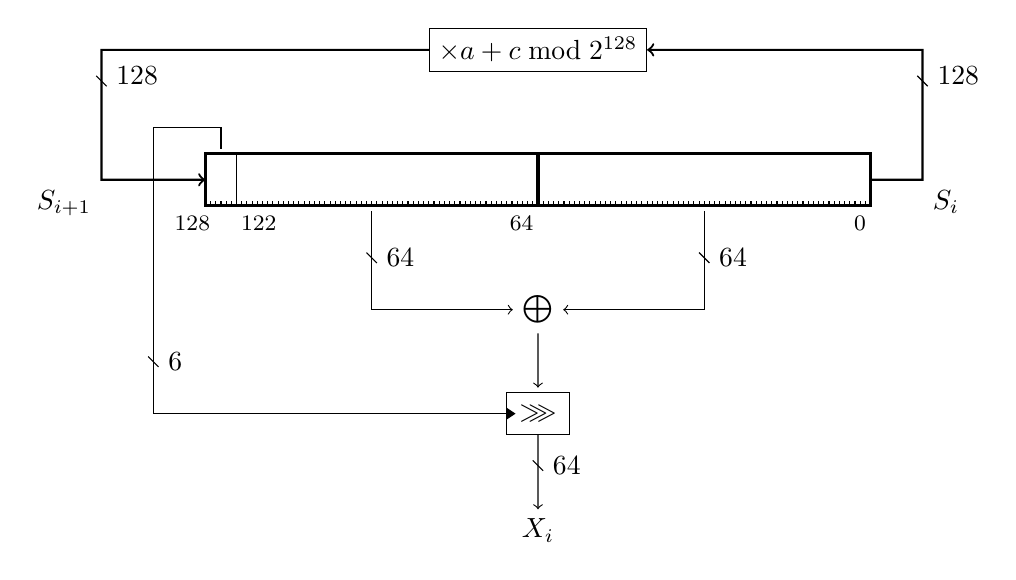
\begin{tikzpicture}[scale=0.66]
%  \draw[red, use as bounding box] (-1.25, -6.75) rectangle (12.8, 2.25);
  
  % S_i

    % bordures
    \draw[very thick]  (0, 0) rectangle (12.8, 1);
    \draw  (0.6, 0) rectangle +(0, 1);
    \draw[very thick]  (6.4, 0) rectangle +(0, 1);
    \foreach \i in {0, 1, ..., 128} \draw (\i/10, 0) -- +(0, 0.1);
    
    % déco autour
    \node[draw] at (6.4, 3) (update) {$\times a + c \bmod 2^{128}$};
    \draw[thick,->] (12.8, 0.5) -- (13.8, 0.5) node[below right] {$S_i$} -- (13.8, 3) -- (update);
    \draw (13.7, 2.5) -- +(0.2, -0.2);
    \path (13.9, 2.5) node[anchor=west] {128};

    \draw[thick,->] (update) -- (-2, 3) -- (-2, 0.5) node[below left] {$S_{i+1}$} -- (0, 0.5);
    \draw (-2.1, 2.5) -- +(0.2, -0.2);
    \path (-1.9, 2.5) node[anchor=west] {128};

    
    \node[font=\footnotesize,anchor=east] at (12.9, -0.33) {0};
    \node[font=\footnotesize,anchor=east] at (6.5, -0.33) {64};
    \node[font=\footnotesize,anchor=west] at (0.5, -0.33) {122};
    \node[font=\footnotesize] at (-0.25, -0.33) {128};
    
    \draw (6.4, -2) node (x) {$\bigoplus$};
    
    \draw[->] (3.2, -0.1) |- (x);
    \draw (3.1, -0.9) -- +(0.2, -0.2);
    \path (3.3, -1) node[anchor=west] {64};
    
    \draw[->] (9.6, -0.1) |- (x);
    \draw (9.5, -0.9) -- +(0.2, -0.2);
    \path (9.7, -1) node[anchor=west] {64};

    \node[minimum width=1.8cm] at (6.4, -4) (r) {$\ggg$};
    \draw (5.8, -3.6) rectangle +(1.2, -0.8);
    \draw[fill=black] (5.8, -4.1) -- (5.95, -4) -- (5.8, -3.9) -- cycle;
    
    \draw (0.3, 1.1) -- (0.3, 1.5) -- (-1, 1.5) -- (-1, -4) -- (5.8, -4);
    \draw (-1.1, -2.9) -- +(0.2, -0.2);
    \path (-0.9, -3) node[anchor=west] {6};

    \draw[->] (x) -- +(0, -1.5);
    \node at (6.4, -6.25) (xi) {$X_i$};
    \draw[->] (6.4, -4.4) -- (xi);

    \draw (6.3, -4.9) -- +(0.2, -0.2);
    \path (6.5, -5) node[anchor=west] {64};
  \end{tikzpicture}
\end{center}
\caption{\textsf{PCG64}: Internal state update and output process.}
\label{pcg128out}
\end{figure}


\section{Algorithm of Frieze \textit{et al}}

\todo{à fusionnier avec la section suivante!}
Pour casser PCG, nous avons utilisé la méthode présentée par Alan M. Frieze, Johan Hastad, Ravi Kannan, Jeffray C. Lagarias et Adi Shamir \cite{Frieze}. Plaçons nous dans le cas simple du Lehmer's generator\cite{Lehmer}. It's a Linear Congruential Generator, a known multiplier $A$, a known modulus $2^128$ and no increment. The outputs $X$ are the 64 upper-bits of $S$. For $n \in \mathbb{N}$, the $n$ firsts internal states form a lattice we will name $\mathcal{L}(A,2^{128},n)$. 
\todo{rajouter ref Lehmer's generator}

This lattice is generated by the matrix :
\begin{equation}
genMatrix =
\begin{pmatrix} 
1 & A & A^2 & \dots & A^{n- 1}\\
0 & M & 0 & \dots & 0\\
0 & 0 & M & \dots & 0\\
\vdots & & & \ddots & \vdots\\
0 & 0 & \dots & 0 & M
\end{pmatrix}
\end{equation}

The idea of this method is to consider a known vector $T$, close to $S$ the internal state we are looking for, and to search for the closest vector in $\mathcal{L}(A,2^{128},n)$. In the case of Lehmer's generator, we use $X * 2^{64}$ as an approximation of $S$.

\todo{preuve que c'est bien le plus proche ici ?}

Pour améliorer les performances de nos algorithmes les plus critiques, nous n'avons dans certains cas pas utilisé d'oracle CVP parfait, mais la méthode du babai-rounding. 

\todo{description babai rounding}
\todo{et preuve ?}

\section{Reconstructing Truncated Geometric Sequences}
\label{sec:geometric}

\todo{à fusionnier avec la section précédente!}
\subsection{The lattice}

One of the key point of the algorithm is, given a modulus \(M\) and a given common ration \(\alpha\), to find a modular geometric progression knowing only the most significant bits of its \(n\) first terms.

We call \(L(\alpha,M,n)\) the set of n-tuples \(U = (u_0,\dots u_{n-1})\) satisfying :

\[u_{i} = \alpha u_{i-1} \mod M \] for all \(i\) in \(\{1,\dots,n-1\}\).


We easily notice that, if \(U\) and \(V\) are in \(L(\alpha,M,n)\), so are \(-U\) and \(U+V\), hence \(L(\alpha,M,n)\) is a lattice.

The lattice \(L(\alpha,M,n)\) is spawned by the lines of the following \(n\times n\) matrix :

\[\begin{pmatrix}
1&\alpha&\alpha^2&\dots&\alpha^{n-1}\\
0&M&0&\dots&0\\
0&0&M&\dots&0\\
\dots&\dots&\dots&\dots&\dots\\
0&0&0&\dots&M\\
\end{pmatrix}\]

We want to find an element \(U\) in the lattice only knowing the most significant bits of each of its coordinates. 


We decompose \(U = T + (T-U)\) where \(T\) contains only the upper bits and \(T-U\) the lowers one. There is no reason for \(T\) to be in the lattice, but as \(T-U\) is small, we know \(T\) is \emph{close} to \(U\).

\subsection{A first way to find U : the Babai's rounding}

We compute \(G\) the LLL-reduction of the generating matrix of \(L(\alpha,M,n)\).

As \(T\) is not an element of the lattice, \(TG^{-1}\) is not an integer vector.

We fix \(r = rounding(TG^{-1}) \), then \(rG\) is an element of the lattice. What can we say about the distance between \(rG\) and \(U\) ?

\begin{align*}
\lVert U - rG \rVert &= \lVert U - (r-TG^{-1} + TG^{-1})G \rVert\\
&= \lVert U - T + (r-TG^{-1})G \rVert\\
&\leqslant \lVert U - T \rVert + \lVert(r-TG^{-1})\rVert \times \lVert G\rVert\\	
\end{align*}

By definition, \(r\) is the closest integer vector to \(TG^{-1}\). But as \(U\) is an element of the lattice, \(UG^{-1}\) is an integer vector. Thus \(r-TG^{-1}\) is shorter than \(UG^{-1}-TG^{-1}\).

Hence :
\begin{align*}
\lVert U - rG \rVert &\leqslant \lVert U - T \rVert + \lVert(r-TG^{-1})\rVert \times \lVert G\rVert\\	
&\leqslant \lVert U - T \rVert + \lVert(UG^{-1}-TG^{-1})\rVert \times \lVert G\rVert\\	
&\leqslant \lVert U - T \rVert + \lVert(U-Y)\rVert \times \lVert G^{-1} \rVert  \times \lVert G\rVert\\
& 	\leqslant \lVert U - T \rVert \times (1 +\lVert G^{-1} \rVert  \times \lVert G\rVert )\\
\end{align*}

If we can prove that the right side \todo{je confonds ma gauche et ma droite et je vous zut :p} of the inequality is smaller than the SVP of G, then wa have proved that \(rG\) is indeed the vector we were searching for.

 \subsection{A second way to find U : using an exact CVP solver}

Solving exactly the CVP is a hard computational problem. But as we do not manipulate quantities too big, we still can use an exact CVP solver.

We know that \(U\) is in the lattice, \(T\) is not and \(|T-U|\) is small. Then we can hope for \(U\) to be the closet vector of \(T\) which is in the lattice : the vector \(U\) may be the solution of \(CVP(L(\alpha,M,n),T)\).

What can we say about \(|CVP(L(\alpha,M,n),T)-U|\) ?

\begin{align*}
|CVP(L(\alpha,M,n),T)-U| &= |CVP(L(\alpha,M,n),T)-T+T-U|\\
& \leqslant |CVP(L(\alpha,M,n),T)-T|+|T-U|\\
\end{align*}

But, as the vector \(U\) is in the lattice and by definition of the CVP, \(|CVP(L(\alpha,M,n),T)-T| \leqslant |T-U| \), hence 
\[|CVP(L(\alpha,M,n),T)-U|\leqslant 2|T-U|\]

If we can prove that the right side of the inequality is smaller than the SVP of the lattice, then wa have proved that \(CVP(L(\alpha,M,n),T)\) is indeed the vector we were searching for.


\section{Warm-up: A Prediction Algorithm for \textsf{PCG64} With Known Increment}

We first consider the easier case where the ``increment'' (the $c$ term in the
definition of the underlying linear congruential generator) is known --- recall
that a default value is specified in case the user of the pseudo-random
generator does not want to provide one.

In this case, reconstructing the 128-bit internal state $S_i$ of the generator
is sufficient to produce the pseudo-random flow with 100\% accuracy (the
generator can also be clocked backwards if necessary, so that the seed can be
easily reconstructed). We therefore focus on reconstructing $S_0$ (the seed)
from $X_0, X_1, X_2, \dots$. A very simple strategy could be the following:
\begin{enumerate}
\item Guess the 64 upper bits of $S_0$.
\item Compute the missing 64 lower bits using~\eqref{eq:output}, with:
\[
   S_0[0:64] = S_0[64:128] \oplus (X_0  \lll S[122:128]).
\]
\item If $X_1$ is computed correctly, output $S_0$.
\end{enumerate}

This requires $2^{64}$ iterations of a loop that does a dozen arithmetic
operations. This is the baseline that we improve upon. An improved
``guess-and-determine'' prediction algorithm is possible, which essentially
amounts to expose a truncated version of the underlying linear congruential
generator, and attack it using the well-known tools. This is possible by
combining the following ingredients:
\begin{itemize}
\item The underlying linear congruential generator uses a power-of-two modulus,
  therefore the $\ell$ low-order bits of $S_{i+1}$ are entirely determined by
  the $\ell$ low-order bits of $S_i$. More precisely, we have:
  \begin{equation}\label{eq:lcg}
    S_{i+1} = aS_i + c \bmod 2^\ell, \qquad \text{for all } 0 \leq \ell \leq 128
  \end{equation}
  Therefore, guessing low-order bits of $S_0$ yields a ``long-term advantage''
  that holds for all subsequent states.

\item Guessing a 6-bit rotation gives access to the XOR of the two halves of the
  internal state. If a part of the state is known, then this transfers existing
  knowledge to the other half.
\end{itemize}

In figure~\ref{fig:Cknown}, we see that guessing $S_0[0:\ell]$ and a few 6-bit
rotations give access to $S_i[58:64+\ell]$ for the corresponding
states. Therefore, looking at $S_i[\ell:64+\ell]$, we are facing a truncated
linear congruential generator on $64$ bits, where we have access to the most
$6+\ell$ bits of each state, for a few consecutive states. This is sufficient to
reconstruct entirely the successive states of this truncated linear congruential
generator. This reveals $S_0[\ell:64+\ell]$, and using~\eqref{eq:output} the
entire $S_0$ can be reconstructed. The precise details follow.

\begin{figure}
\begin{center}
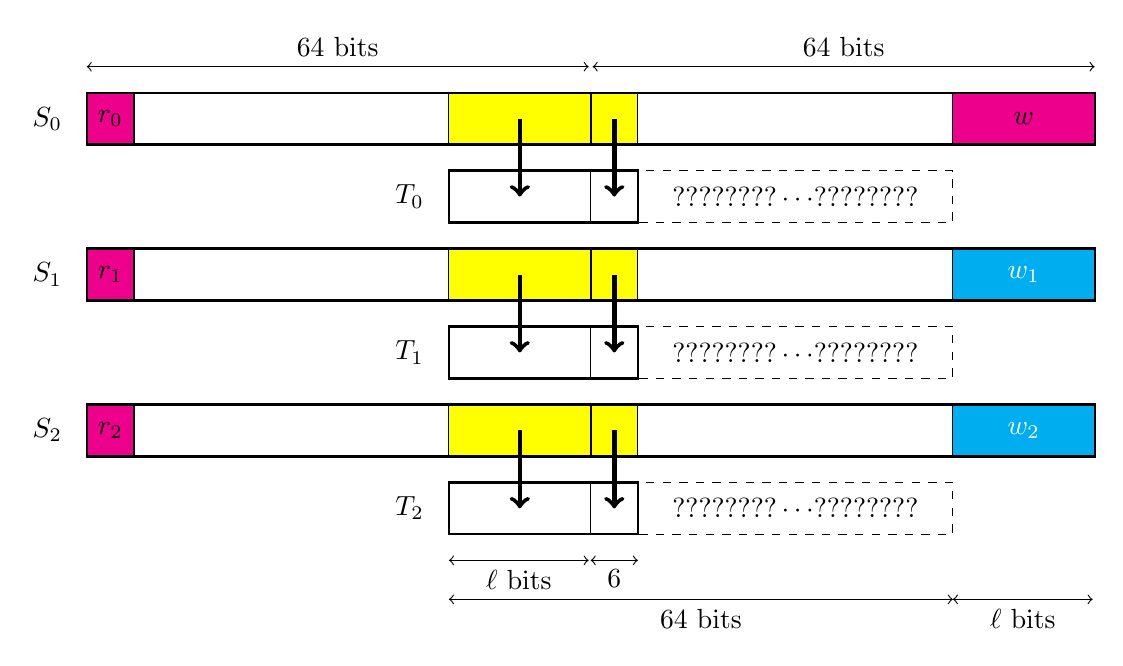
\begin{tikzpicture}[yscale=0.66]
  \path[red, use as bounding box] (-0.75, -9.5) rectangle (12.8, 2.25);
  
  % S_0
  \begin{scope}
    % remplissage
    \fill[fill=Yellow] (4.6, 0) rectangle +(2.4, 1);
    \fill[fill=magenta] (0, 0) rectangle node {$r_0$} +(0.6, 1);
    \fill[fill=magenta] (11, 0) rectangle node {$w$} +(1.8, 1);
    
    % bordures
    \draw[thick]  (0, 0) rectangle (12.8, 1);
    \draw  (0.6, 0) rectangle +(0, 1);
    \draw[thick]  (6.4, 0) rectangle +(0, 1);
    \draw  (7.0, 0) rectangle +(0, 1);
    \draw  (4.6, 0) rectangle +(0, 1);
    \draw  (11, 0) rectangle +(0, 1);
    
    % déco autour
    \node at (-0.5, 0.5) {$S_0$};
    \draw[<->] (0, 1.5) -- node[above] {64 bits} +(6.375, 0);
    \draw[<->] (6.425, 1.5) -- node[above] {64 bits} +(6.375, 0);
  \end{scope}

  % T_0
  \begin{scope}[xshift=4.6cm, yshift=-1.5cm]    
    \draw[dashed]  (0, 0) rectangle +(6.4, 1);
    \draw[thick]  (0, 0) rectangle +(2.4, 1);
    \draw[]  (1.8, 0) rectangle +(0, 1);
    \path (2.4, 0) rectangle node {$???????? \cdots ????????$} (6.4, 1);

    % déco
    \node at (-0.5, 0.5) {$T_0$};
  \end{scope}

  % flèches S_i --> T_i
  \draw[ultra thick,->] (5.5, 0.5) -- +(0, -1.5);
  \draw[ultra thick,->] (6.7, 0.5) -- +(0, -1.5);

  
  %%%%%%%%%

  
  % S_1
  \begin{scope}[yshift=-3cm]
    % remplissage
    \fill[fill=Yellow] (4.6, 0) rectangle +(2.4, 1);
    \fill[fill=magenta] (0, 0) rectangle node {$r_1$} +(0.6, 1);
    \fill[fill=cyan] (11, 0) rectangle node[text=white] {$w_1$} +(1.8, 1);
    
    % bordures
    \draw[thick]  (0, 0) rectangle (12.8, 1);
    \draw  (0.6, 0) rectangle +(0, 1);
    \draw[thick]  (6.4, 0) rectangle +(0, 1);
    \draw  (7.0, 0) rectangle +(0, 1);
    \draw  (4.6, 0) rectangle +(0, 1);
    \draw  (11, 0) rectangle +(0, 1);
    
    % déco autour
    \node at (-0.5, 0.5) {$S_1$};

    % flèches S_i --> T_i
    \draw[ultra thick,->] (5.5, 0.5) -- +(0, -1.5);
    \draw[ultra thick,->] (6.7, 0.5) -- +(0, -1.5);
  \end{scope}

  % T_1
  \begin{scope}[xshift=4.6cm, yshift=-4.5cm]    
    \draw[dashed]  (0, 0) rectangle +(6.4, 1);
    \draw[thick]  (0, 0) rectangle +(2.4, 1);
    \draw[]  (1.8, 0) rectangle +(0, 1);
    \path (2.4, 0) rectangle node {$???????? \cdots ????????$} (6.4, 1);

    % déco
    \node at (-0.5, 0.5) {$T_1$};
  \end{scope}

  %%%%%%%%%%%%%

  
  % S_2
  \begin{scope}[yshift=-6cm]
    % remplissage
    \fill[fill=Yellow] (4.6, 0) rectangle +(2.4, 1);
    \fill[fill=magenta] (0, 0) rectangle node {$r_2$} +(0.6, 1);
    \fill[fill=cyan] (11, 0) rectangle node[text=white] {$w_2$} +(1.8, 1);
    
    % bordures
    \draw[thick]  (0, 0) rectangle (12.8, 1);
    \draw  (0.6, 0) rectangle +(0, 1);
    \draw[thick]  (6.4, 0) rectangle +(0, 1);
    \draw  (7.0, 0) rectangle +(0, 1);
    \draw  (4.6, 0) rectangle +(0, 1);
    \draw  (11, 0) rectangle +(0, 1);
    
    % déco autour
    \node at (-0.5, 0.5) {$S_2$};
    
    % flèches S_i --> T_i
    \draw[ultra thick,->] (5.5, 0.5) -- +(0, -1.5);
    \draw[ultra thick,->] (6.7, 0.5) -- +(0, -1.5);
  \end{scope}

  % T_2
  \begin{scope}[xshift=4.6cm, yshift=-7.5cm]    
    \draw[dashed]  (0, 0) rectangle +(6.4, 1);
    \draw[thick]  (0, 0) rectangle +(2.4, 1);
    \draw[]  (1.8, 0) rectangle +(0, 1);
    \path (2.4, 0) rectangle node {$???????? \cdots ????????$} (6.4, 1);

    % déco
    \node at (-0.5, 0.5) {$T_2$};
    \draw[<->] (0, -0.5) -- node[below] {$\ell$ bits} +(1.775, 0);
    \draw[<->] (1.8, -0.5) -- node[below] {6} +(0.6, 0);
    \draw[<->] (0, -1.25) -- node[below] {64 bits} +(6.4, 0);
    \draw[<->] (6.4, -1.25) -- node[below] {$\ell$ bits} +(1.775, 0);
  \end{scope}
\end{tikzpicture}

\end{center}
\caption{A guess-and-determine algorithm to reconstruct the first internal state
  $S_0$. Magenta bits are guessed; cyan bits are obtained using the linear
  congruence relation~\eqref{eq:lcg} modulo $2^\ell$; yellow bits are obtained
  from the output and the guessed rotations using~\eqref{eq:output}.}
\label{fig:Cknown}
\end{figure}

Set $S_i' = S_i - S_0[0:\ell] a^i - c \sum_{j=0}^{i-1} a^i$. The sequence
$(S'_i)$ describe the internal states we would observe if $c=0$ and
$S_0[0:\ell] = 0$. It is easy to check that $S'_{i} = a^i (S_0 - S_0[0:\ell])$,
and therefore the successive $S'_i$'s follow a geometric progression. % Indeed :
% \begin{align*}
% S_i &= a S_{i-1} + c\\
%     &= a^2 S_{i-2} + (a + 1) c \\
%     &\vdots  \\
%     &= a^i S_0  + c \sum_{j=0}^{i-1} a^i \\
%   S'_i  &= S_i - c \sum_{j=0}^{i-1} a^i - S_0[0:\ell] a^i \\
%     &= a^i (S_0 - S_0[0:\ell])
% \end{align*}
The $\ell$ low-order bits of $S_0 - S_0[0:\ell]$ are all zero by construction;
therefore set $T_i = \left(S'_i / 2^\ell\right) \bmod 2^{64}$ (the division by
$2^\ell$ is exact). It follows that the $(T_i)$ is also a geometric progression
with common ratio $a$, and we have access to the $\ell+6$ high order bits of
$T_i$ if we guess the $i$-th rotation. We have seen in
section~\ref{sec:geometric} that 19 known bits on 3 consecutive outputs are
sufficient for a deterministic reconstruction of the full sequence. Therefore,
we guess 19 low-order bits of the state and three consecutive rotations.

Therefore, the algorithm that reconstructs the internal state of the
\textsf{PCG64} generator with known increment proceeds as follows:

\begin{center}\noindent\framebox{
  \begin{minipage}{0.95\textwidth}
    \algbegin Algorithm K (State reconstruction with known
    increment). Reconstruct $S_0$ from three consecutive outputs $X_j$
    ($0 \leq j < 3$). In all steps of the algorithm, we have $j= 0, 1, 2$.

\algstep K1. [Guess state] For each $0 \leq w < 2^{19}$, set $w_j = a^j w \bmod 2^{19}$ and do steps K2--K0.

\algstep K2. [Guess rotations] For each $0 \leq r_0, r_1, r_2 < 64$, do steps K3--K9.

\algstep K3. [Undo rotations] Set $Y_j \gets X_j \lll r_j$. % ($Y_j$ is the $j$-th output on which the rotation has been undone).

\algstep K4. [Build $T$] Set $T_j \gets \left(r_j \oplus Y_j[58:64]\right) \oplus \bigl( 64 \cdot \left(w_j \oplus Y_j[0:19]\right)\bigr)$.

\algstep K5. [Shift $T$] Set $T'_j \gets  T_j - (a^j w + c \sum_{k = 0}^j a^k)[58:83]$

\algstep K6. [Truncated LCG] Set $(U_0, U_1, U_2) \gets \left\lfloor (T_0, T_1, T_2) \cdot 2^{39} \cdot \widetilde G^{-1} \right\rceil \cdot \widetilde G$.

\algstep K7. [Reconstruct $S_0$] Set $\widehat S_0[0:64] \gets w + 2^{19} \cdot U_0[0:45]$ and $\widehat S_0[64:128] \gets S_0[0:64] \oplus Y_0$.

\algstep K8. [Recompute $Y_1$] Set $\widehat S_1 \gets a \widehat S_0 + c$ and $\widehat Y_1 = \widehat S_1[0:64] \oplus \widehat S_1[64:128]$.

\algstep K9. [Check] If $\widehat{Y}_1 = Y_1$, then output $\widehat S_0$ as a candidate internal state.
\end{minipage}
}
\end{center}

\subsection{preuve cas facile}

The vector \(S'\) has been constructed such that it is in \(L(A,2^{128},n)\) and its \(\ell\) lower bits are zero.

We call \(U\) the truncated vector : \(S'[\ell,64+\ell]\). We notice that \(U\) is in \(L(A,2^{64},n)\).

We consider the case were we successfully guessed the 6 upper bits of each \(S_i\) and the \(\ell\) lower bits of \(S_0\). Then we know the \(6+\ell\) upper bits of \(U\).

(maybe dessin)


We consider the vector \(T'\) computed in step (numerodelastepenquestion). To recover \(U\), we use the Babai's rounding explain in section (insererlasection) on \(T'\) and \(L(A,2^{64},n)\).

As \(U\) and \(T'\) have exactly the same \(6+\ell\) upper bits  know that \(\lVert U-T \rVert \leqslant \sqrt{n2^{2(58-l)}}\).

So, to be sure that our algorithm return the vector \(U\), we need to find sets of parameters \((n,\ell)\) such that :	 

\[\sqrt{n2^{2(58-\ell)}} \times (1 +\lVert G^{-1} \rVert  \times \lVert G\rVert) \leqslant \lVert SVP(L(A,2^{64},n))\rVert \]

\begin{itemize}
	\item For \(n=3\)
	
	\(G = \begin{pmatrix}
	-1241281756092&3827459685972&-728312298332\\
	-5001120657083&-2117155768935&5479732607037\\
	8655886039732&3303731088004&6319848582548\\
	\end{pmatrix}\)
	
	\(\lVert G \rVert \times \lVert G^{-1} \rVert = 2.869065991049632\)
	
	\(\lVert SVP(G) \rVert = 4.08909120094543e{^12}\)
	
	Hence, the smallest l such that the inequality is satisfied is \(\ell = 19\) %17 avec borne CVP
	
	\item For \(n=4\)
	
	\(G = \begin{pmatrix}
	-186304953996472&-126056243766680&7937589136904&93078431381544\\
	-216211368070119&99587582169277&-214303762177807&-1707551230219\\
	110964501361298&-5646098666150&-268280113597118&149382085707466\\
	131252974561432&-233919070109448&-98716819647784&-134620659538888\\
	\end{pmatrix}\)
	
	\(\lVert G \rVert \times \lVert G^{-1} \rVert = 2.060717188416003\)
	
	\(\lVert SVP(G) \rVert = 2.43569932844650e^{14}\)
	
	Hence, the smallest l such that the inequality is satisfied is \(\ell = 13\) %11 avec borne CVP
	
	\item For \(n=5\)
	
	\(\lVert G \rVert \times \lVert G^{-1} \rVert = 3.7692142154392747\)
	
	\(\lVert SVP(G) \rVert = 1.71669732658884e^{15}\)
	
	Hence, the smallest l such that the inequality is satisfied is \(\ell = 11\)  %9 avec borne CVP
	
	\item For \(n=6\)
	
	\(\lVert G \rVert \times \lVert G^{-1} \rVert = 2.6925925483728537\)
	
	\(\lVert SVP(G) \rVert =1.02550589786192e^{16}\)
	
	Hence, the smallest l such that the inequality is satisfied is \(\ell = 8\) %7 avec borne CVP
\end{itemize}

[insert here] attack predicting algo description.

\begin{theorem}
  The algorithm described above works with probability.... in time ...
\end{theorem}

\section{Predicting PCG with Unknown Increment}
We can't use the same algorithm for the general case. We don't known $C$, so we used an other geometric reduction.
$(\Delta S_{i+1}S_i)_i$ est un suite géométrique de raison $A$.

On calcule préalablement les matrices $G$ et $G^{-1}$.

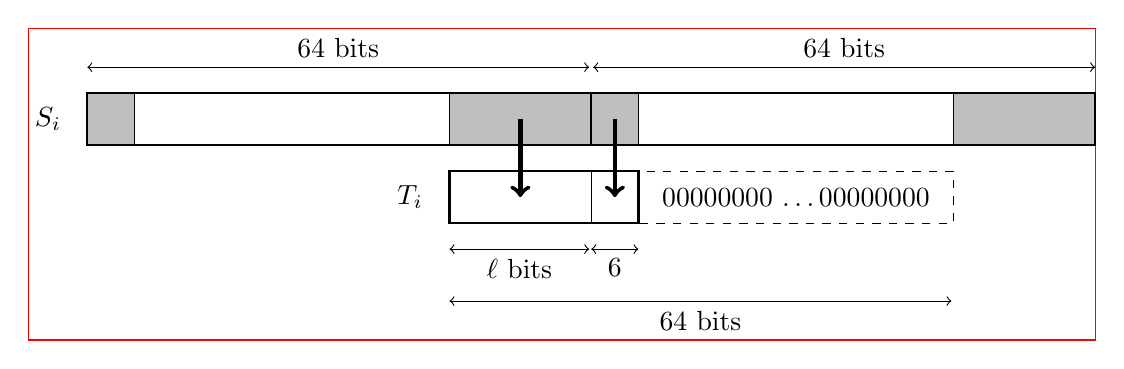
\begin{tikzpicture}[yscale=0.66]
  \draw[red, use as bounding box] (-0.75, -3.75) rectangle (12.8, 2.25);
  
  % S_i
  \begin{scope}
    % remplissage
    \fill[fill=lightgray] (4.6, 0) rectangle +(2.4, 1);
    \fill[fill=lightgray] (0, 0) rectangle +(0.6, 1);
    \fill[fill=lightgray] (11, 0) rectangle +(1.8, 1);
    
    % bordures
    \draw[thick]  (0, 0) rectangle (12.8, 1);
    \draw  (0.6, 0) rectangle +(0, 1);
    \draw[thick]  (6.4, 0) rectangle +(0, 1);
    \draw  (7.0, 0) rectangle +(0, 1);
    \draw  (4.6, 0) rectangle +(0, 1);
    \draw  (11, 0) rectangle +(0, 1);
    
    % déco autour
    \node at (-0.5, 0.5) {$S_i$};
    \draw[<->] (0, 1.5) -- node[above] {64 bits} +(6.375, 0);
    \draw[<->] (6.425, 1.5) -- node[above] {64 bits} +(6.375, 0);
  \end{scope}

  % T_i
  \begin{scope}[xshift=4.6cm, yshift=-1.5cm]    
    \draw[dashed]  (0, 0) rectangle +(6.4, 1);
    \draw[thick]  (0, 0) rectangle +(2.4, 1);
    \draw[]  (1.8, 0) rectangle +(0, 1);
    \path (2.4, 0) rectangle node {00000000 \dots 00000000} (6.4, 1);

    % déco
    \node at (-0.5, 0.5) {$T_i$};
    \draw[<->] (0, -0.5) -- node[below] {$\ell$ bits} +(1.775, 0);
    \draw[<->] (1.8, -0.5) -- node[below] {6} +(0.6, 0);
    \draw[<->] (0, -1.5) -- node[below] {64 bits} +(6.375, 0);
  \end{scope}

  % flèches S_i --> T_i
  \draw[ultra thick,->] (5.5, 0.5) -- +(0, -1.5);
  \draw[ultra thick,->] (6.7, 0.5) -- +(0, -1.5);
  
\end{tikzpicture}

\subsection{Part 1 : Premier filtre}
Pour tous les $r_i$, les $S_0[0 : \ell]$ et les $C[0 : \ell]$ possibles:
\begin{enumerate}
  \item On récupère le $T$  correspondant à nos suppositions. On calcule $\Delta T$ :
  \begin{equation}
    \Delta T_i = (S_{i+1}[58 : 64 + \ell] - S_i[58 : 64 + \ell] - (S_0[0:\ell] * (A^{i+1} - A^i) + C[0:\ell] * A^i )[58 : 64 + \ell]) * 2^{64 - l - 6}
  \end{equation}
  Ou plus simplement $\Delta T_i = T'_{i+1} - T'_{i}$ avec $T'$ dont on aurait soustrait la composante en $C[0:\ell]$ et non en $C$.

  \item We get the correspondant $\Delta S_0S_1[0 : 64 + \ell]$ by using the babai rounding technique on $\Delta T$ using $G$ and $G^{-1}$.

  \item On teste s'il existe pour l'itération suivante au moins une rotation $r_n$ cohérente avec le $\Delta T$ trouvé. Pratiquement, pour chacune des 64 $r_n$ possibles, on teste si :
  \begin{align}
     \Delta S_0S_n[0:l] &= S_0[64:64 + \ell] \oplus \mathtt{ROT(X_n , 64 - r_n)[0:\ell]}\\
     r_n &= S_0[58:64] \oplus \mathtt{ROT(X_n , 64 - r_n)[58:64]}
  \end{align}
  Si un de ces égalité n'est pas vérifiée, la solution n'est pas retenue, on passe à la prochaine itération.

  \item On répète la dernière opération encore 3 fois.
\end{enumerate}
Cette première partie de l'algorithme comporte l'énorme majorité du temps de calcul, c'est donc sur elle que doit se porter la recherche de performance.


\subsection{Part 2 : Récupération de la différence complète et deuxième filtre}
On calcule préalalement H matrice génératrice du réseau $\mathcal{L}(A,2^{128 - \ell},m)$ réduite par la méthode LLL.
On a récupéré de la Part 1 une série de $S_0[0 : \ell]$, $r_i$ (i = 0, ..., n) et $C[0 : \ell]$ parmi lequels se trouve notre solution.
\begin{enumerate}
  \item recupérer toutes les $r_i$ possibles, pour $n \leq i \leq m$  par la même méthode que l'étape 3 de la Part 1, répétée $m-n$ fois. On garde en mémoire toutes les rotations possiles.
  \item Pour chacune des $r$ possibles
  \begin{enumerate}
    \item We cumpute $r'$ et $\Delta r$ avec le même méthode que pour $\Delta T$ : 
    \begin{align}
      r'_i = r_i - (A^i*S_0[0 : \ell] + C[0 : \ell] * \sum_{j = 0}^i A^j)[64 - 6 : 64 + \ell])[122 : 128]
      \Delta r_i &= r_{i+1} - r_i
    \end{align}

    \item We get the correspondant $\Delta S'_0S'_1$ ($S'$ dont on aurait retiré que la composante en $C[0 : \ell]$ et non en $C$ entier) computing $\texttt{CVP}(r * 2^{128 - \ell}, \mathcal{L}(A,2^{128 - \ell},m))$. We use the fpylll python library CVP function. On stocke le $DS_0S_1$ correspondant.

    \item \todo{parler du problème de retenue étrange}
    
  \end{enumerate}
\end{enumerate}

\subsection{preuve cas difficile}
\todo{À ranger au bon endroit}
% Babai ça marche pas (genre zero)

The vector \(S'\) has been constructed such that it is in \(L(A,2^{128},n)\) and its \(\ell\) lower bits are zero.

We call \(U\) the truncated vector : \(S'[\ell,128]\). We notice that \(U\) is in \(L(A,2^{128-\ell},n)\).

We consider the case were we successfully guessed the 6 upper bits of each \(S_i\) and the \(\ell\) lower bits of \(S_0\). Then we know the 6 upper bits of \(U\).

(maybe dessin)


We consider the vector \(T'\) computed in step (numerodelastepenquestion). To recover \(U\), we use an exact CVP solver as explain in  (insererlasection) on \(T'\) and \(L(A,2^{128-\ell},n)\).

As \(U\) and \(T'\) have exactly the same \(6\) upper bits  know that \(\lVert U-T \rVert \leqslant \sqrt{n2^{2(128-6-\ell)}}\).

So, to be sure that our algorithm return the vector \(U\), we need to find sets of parameters \((n,\ell)\) such that :	 

\[2\sqrt{n}^{(128-6-\ell)} \leqslant \lVert SVP(L(A,2^{128-\ell},n))\rVert \]

\begin{itemize}
	\item For \(\ell=11\), the smallest \(n\) we need is 39.
	
	\item For \(\ell=12\), the smallest \(n\) we need is 38.
	
	\item For \(\ell=13\), the smallest \(n\) we need is again 38 .
	
\end{itemize} 

\begin{theorem}
  The algorithm described above works with probability.... in time ...
\end{theorem}

\section{Implementation of the Predictor and Practical Results}

\section{Conclusion}

\bibliographystyle{alpha}
\bibliography{biblio}

%\appendix

\end{document}

% Charles' emacs magic commands
%%% Local Variables:
%%% TeX-command-extra-options: "-shell-escape"
%%% ispell-local-dictionary: "english"
%%% eval: (flyspell-mode 1)
%%% eval: (reftex-mode 1)
%%% End:
